\documentclass[12pt]{article}
% Packages
\usepackage[utf8]{inputenc}
\usepackage[T1]{fontenc}
\usepackage[margin=1in]{geometry}
\usepackage{amsmath, amsthm, amsfonts, amssymb}
\usepackage{mathrsfs}           % \mathscr font.
\usepackage{setspace}

\usepackage[UKenglish]{babel}% http://ctan.org/pkg/babel
\usepackage[UKenglish]{isodate}% http://ctan.org/pkg/isodate

\usepackage[colorlinks=true,
    linkcolor=red,
    citecolor=red,
    urlcolor=red,
    breaklinks]{hyperref}
\usepackage{graphicx}
\usepackage{booktabs}
\usepackage{xcolor}
\usepackage[style = authoryear, autocite=inline, doi=false,isbn=false,url=false]{biblatex}
% \usepackage{libertine}

% \usepackage[sf]{titlesec} % make section headings \sffamily

% Header styling
% make headers \sffamily
% \newpagestyle{main}[\sffamily]{
%     \sethead{\thepage}{}{\sectiontitle}
%     }
% \pagestyle{main}
\usepackage{titling}
% make titling elements \sffamily
\pretitle{\begin{center}\sf \LARGE}
\preauthor{\begin{center}
            \large \lineskip 0.5em%
            \begin{tabular}[t]{c}}
\predate{\begin{center}\large}
\usepackage{abstract}
% make abstract title \sffamily
% \titleformat{\section}[block]{\Large \bf \sffamily}{\thesection}{1em}{}
\usepackage{caption}
\captionsetup{labelfont = bf}

\usepackage{longtable}
\usepackage{dcolumn}
\usepackage[toc,page,header]{appendix}
\usepackage{minitoc}
\usepackage{siunitx}
\sisetup{
    detect-all,
    round-integer-to-decimal = true,
    group-digits             = true,
    group-minimum-digits     = 4,
    group-separator          = {\,},
    table-align-text-pre     = false,
    table-align-text-post    = false,
    input-signs              = + -,
    input-symbols            = {*} {**} {***},
    input-open-uncertainty   = ,
    input-close-uncertainty  = ,
    retain-explicit-plus,
    parse-numbers = false
}
\newcolumntype{d}[1]{D..{#1}}
% Make the "Part I" text invisible
\renewcommand \thepart{}
\renewcommand \partname{}


% Define symbols and maths shortcuts
\DeclareRobustCommand{\bbone}{\text{\usefont{U}{bbold}{m}{n}1}}
\DeclareMathOperator{\EX}{\mathbb{E}} % expected value
\DeclareMathOperator{\V}{\mathbb{V}}
\DeclareMathOperator{\Prob}{\mathbb{P}}
\newcommand*{\trans}{^{\mathsf{T}}} %matrix transpose



\usepackage{biblatex}
\addbibresource{UKCareers.bib}

\usepackage[]{booktabs}

\setlength\labelsep{0pt}

\title{Car Fuel Consumption}
\author{Tobias Nowacki\thanks{Ph.D. Candidate in Political Science, Stanford University, Calif., USA. \texttt{tnowacki@stanford.edu}}}


% Begin Document
\begin{document}

\maketitle

\begin{abstract}
Cars with more horsepower also consume more fuel.
\end{abstract}


\doublespacing

\clearpage

\section{Evidence}

\parencite[][]{eggers2014a}

\subsection{Tables are great}

\begin{table}[tb]
    \caption{This is my main evidence}
    \label{tab:tablename}
    \centering

    \begin{tabular}{lcc}
    \toprule
    \textbf{column 1} & \textbf{column 2} & \textbf{column 3} \\
    \hline
        24 & 37.4 & -100.8 \\
    \bottomrule
    \end{tabular}
\end{table}

The following figure shows this:

\begin{equation}
\label{eq:integral}
\int_a^b = x^2 dx
\end{equation}

As we see per Equation \ref{eq:integral}


$lim_{h \rightarrow 0} \frac{f(x + h) - f(x)}{h} = f'(x)$


Hello. My name is toby. I don't know what I'm doing.


\begin{figure}[tb]
  \centering
  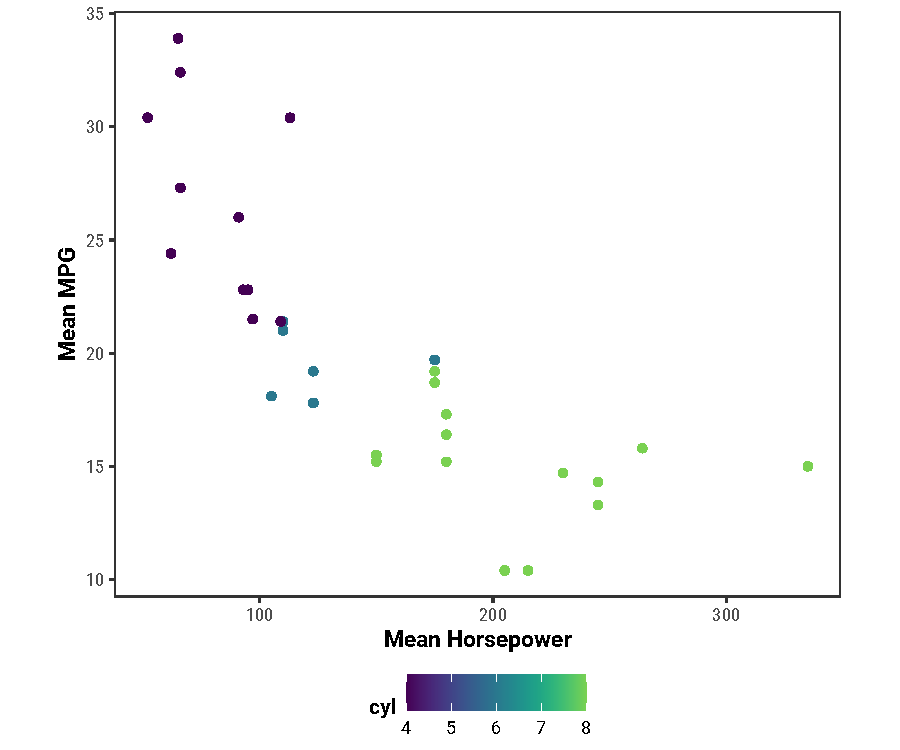
\includegraphics[]{output/plot1}
  \caption{Sample of cars with their horse power and fuel efficiency.}
  \label{fig:figure1}
\end{figure}

\printbibliography


\end{document}
